% ============================================================
\section{Actividad 4: Herramienta de clasificación mono/multifractal}
% ============================================================

Se desarrolla una herramienta en MATLAB que, dada una secuencia discreta,
determina si es monofractal o multifractal. El algoritmo opera en dos etapas
basadas en el $R^2$ del ajuste lineal:

\begin{enumerate}[nosep]
    \item \textbf{Verificación de LRD} ($R^2_{\text{VT}} \geq 0{,}85$): se
          ajusta una recta al diagrama varianza--tiempo. Si el ajuste es pobre,
          la muestra se descarta como \emph{no clasificable}.
    \item \textbf{Clasificación fractal} ($R^2_{\tau} \geq 0{,}90$): se
          obtienen los exponentes de escala $\tau(q)$ con \texttt{dwtleader}.
          Si $\tau(q)$ es lineal, la muestra es monofractal; si presenta
          curvatura, es multifractal.
\end{enumerate}

% ────────────────────────────────────────────────────────────
\subsection{Diagrama de flujo}

La Figura~\ref{fig:flujo-clasificador} presenta el algoritmo implementado.

\begin{figure}[H]
\centering
\resizebox{\textwidth}{!}{%
\begin{tikzpicture}[
    startstop/.style={
        ellipse, draw=black!80, fill=blue!8,
        minimum width=2.4cm, minimum height=0.9cm,
        font=\bfseries\small, align=center, thick
    },
    process/.style={
        rectangle, draw=black!80, fill=white,
        minimum width=3.5cm, minimum height=1cm,
        font=\small, align=center, thick, rounded corners=2pt
    },
    decision/.style={
        diamond, draw=black!80, fill=orange!8,
        minimum width=2.8cm, minimum height=1.4cm,
        font=\small, align=center, thick, aspect=2.4
    },
    io/.style={
        trapezium, trapezium left angle=70, trapezium right angle=110,
        draw=black!80, fill=green!6,
        minimum width=2.8cm, minimum height=0.9cm,
        font=\small, align=center, thick
    },
    result/.style={
        rectangle, draw=black!80, fill=blue!10,
        minimum width=3cm, minimum height=0.9cm,
        font=\small\bfseries, align=center, thick, rounded corners=2pt
    },
    arr/.style={-Stealth, thick, black!70},
    lbl/.style={font=\footnotesize\bfseries, text=black!70},
    node distance=1.1cm
]

% ── Columna principal ──
\node[startstop]                       (inicio) {Inicio};
\node[io, below=of inicio]            (input)  {Vector con\\la muestra};
\node[process, below=of input]         (calcvt) {Usar \texttt{vt}\\en la muestra};

\node[decision, below=1.4cm of calcvt] (decvt)  {¿Ajuste\\lineal?\\{\scriptsize $R^2_{\text{VT}} \geq 0{,}85$}};

% ── Rama Sí (derecha) ──
\node[process, right=3.8cm of decvt]   (geth)   {$H \leftarrow$ \texttt{vt2(muestra)}};
\node[process, below=of geth]          (dwt)    {Calcular $\tau(q)$\\con \texttt{dwtleader}};

\node[decision, below=1.4cm of dwt]    (dectau) {¿Ajuste\\lineal?\\{\scriptsize $R^2_{\tau(q)} \geq 0{,}90$}};

% ── Clasificaciones ──
\node[result, right=2.8cm of dectau]   (mono)   {Monofractal};
\node[result, left=2.8cm of dectau]    (multi)  {Multifractal};

% ── Graficación y salida ──
\node[process, below=2.8cm of dectau]  (graf)   {Graficar VT, LD,\\$\tau(q)$, $D(h)$};
\node[io, below=of graf]               (output) {$H$, Clasificación};
\node[startstop, below=of output]      (fin1)   {Fin};

% ── Rama No del VT (izquierda) ──
\node[process, left=3.8cm of decvt]    (grafvt) {Graficar VT};
\node[result, below=of grafvt]         (noclas) {No clasificable};
\node[startstop, below=of noclas]      (fin2)   {Fin};

% ── Flechas ──
\draw[arr] (inicio) -- (input);
\draw[arr] (input)  -- (calcvt);
\draw[arr] (calcvt) -- (decvt);
\draw[arr] (decvt)  -- node[lbl, above] {Sí} (geth);
\draw[arr] (decvt)  -- node[lbl, above] {No} (grafvt);
\draw[arr] (geth)   -- (dwt);
\draw[arr] (dwt)    -- (dectau);
\draw[arr] (dectau) -- node[lbl, above] {Sí} (mono);
\draw[arr] (dectau) -- node[lbl, above] {No} (multi);
\draw[arr] (mono.south)  |- (graf.east);
\draw[arr] (multi.south) |- (graf.west);
\draw[arr] (graf)   -- (output);
\draw[arr] (output) -- (fin1);
\draw[arr] (grafvt) -- (noclas);
\draw[arr] (noclas) -- (fin2);

\end{tikzpicture}
}%
\caption{Diagrama de flujo del clasificador mono/multifractal.}
\label{fig:flujo-clasificador}
\end{figure}

% ────────────────────────────────────────────────────────────
\subsection{Validación}

Se generan muestras de $2^{17}$ datos con \texttt{wfbm} (monofractal) y
\texttt{betamwm} (multifractal) para validar la herramienta. Las
Figuras~\ref{fig:val-mono} y~\ref{fig:val-multi} muestran los resultados para
$H = 0{,}8$.

\begin{figure}[H]
    \centering
    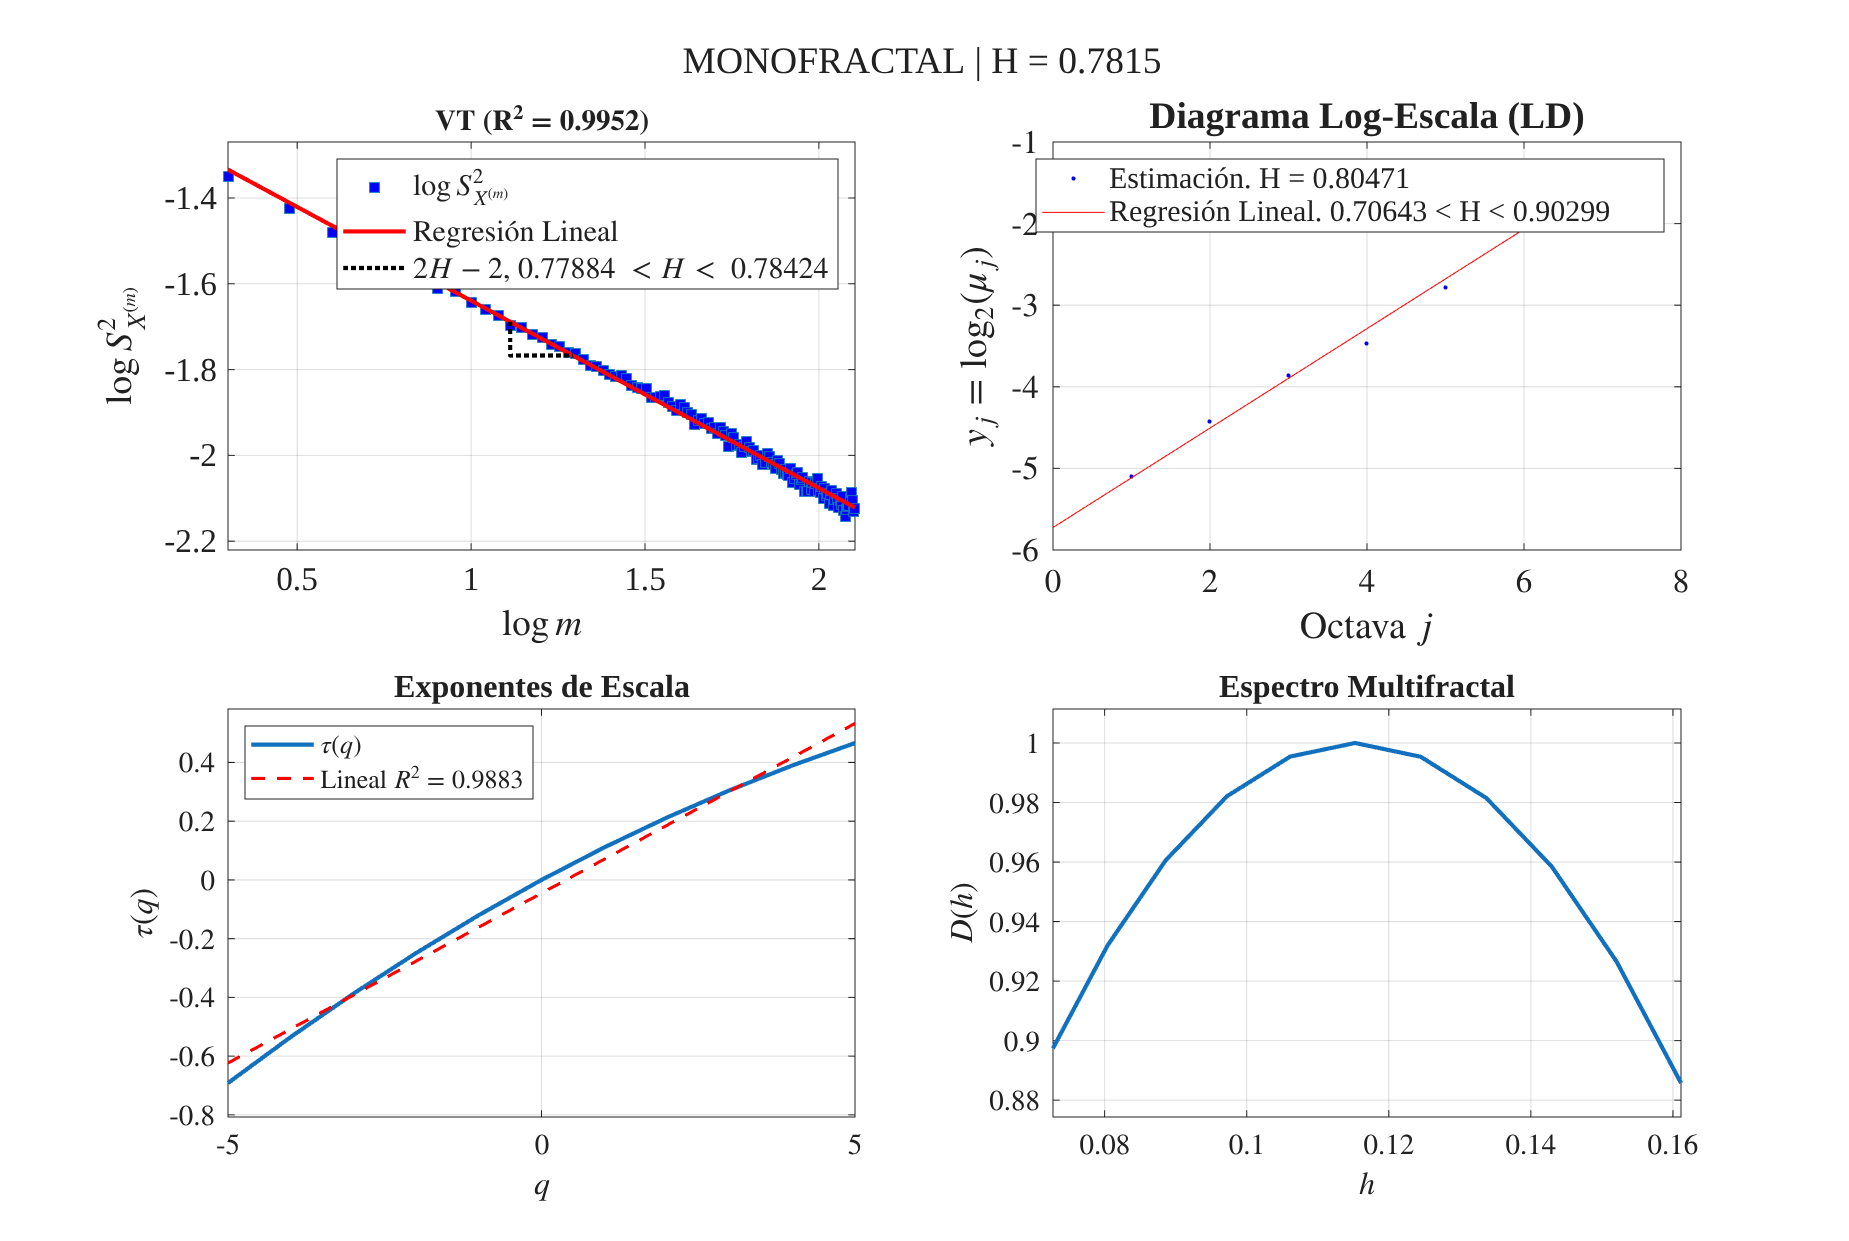
\includegraphics[width=\textwidth]{assets/plots/mono.png}
    \caption{Muestra monofractal (\texttt{wfbm}, $H = 0{,}8$): $\tau(q)$ es
             lineal ($R^2_{\tau} = 0{,}9883$) y $D(h)$ se concentra en un rango
             estrecho.}
    \label{fig:val-mono}
\end{figure}

\begin{figure}[H]
    \centering
    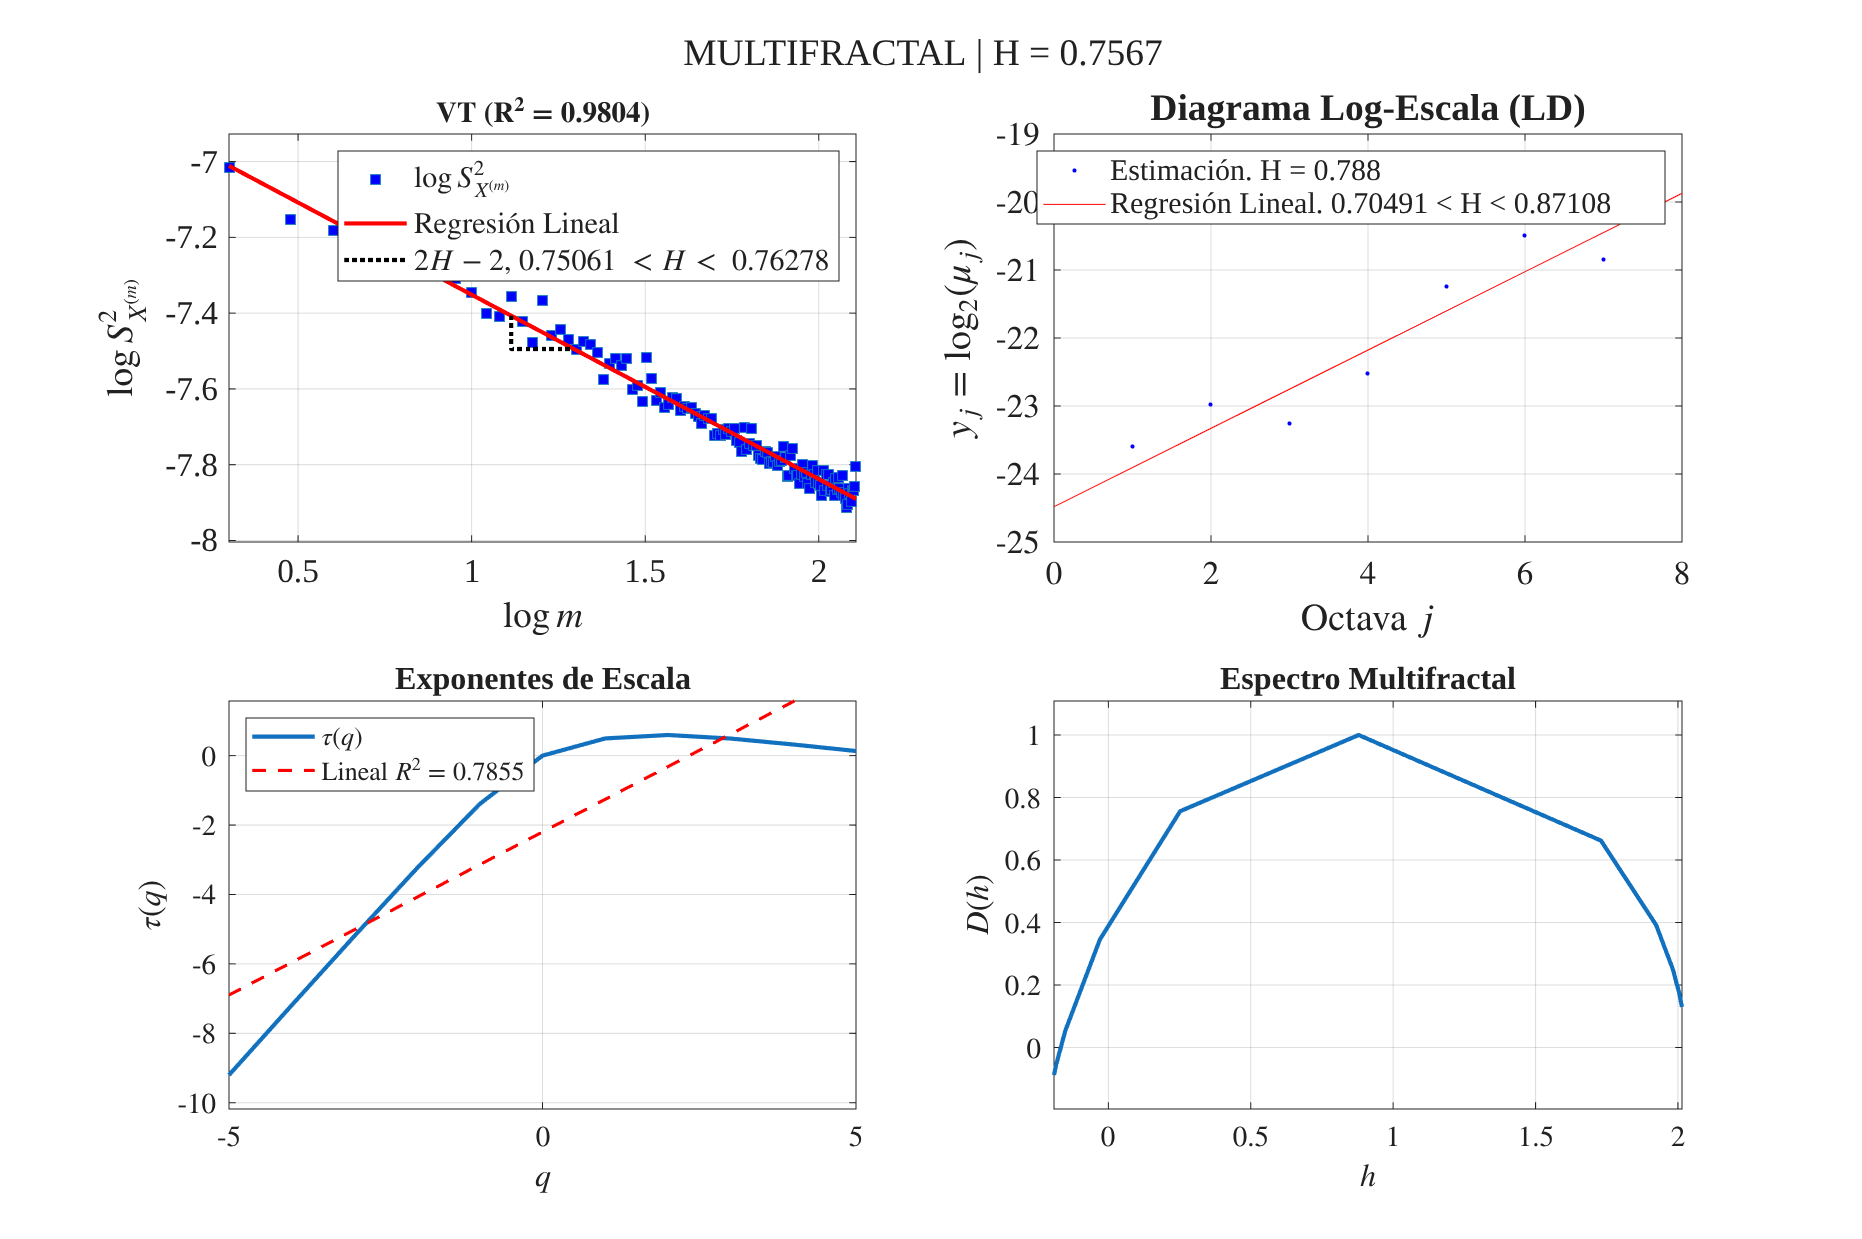
\includegraphics[width=\textwidth]{assets/plots/multi.png}
    \caption{Muestra multifractal (\texttt{betamwm}, $H = 0{,}8$): $\tau(q)$
             presenta curvatura ($R^2_{\tau} = 0{,}7855$) y $D(h)$ tiene forma
             de campana.}
    \label{fig:val-multi}
\end{figure}

La Tabla~\ref{tab:barrido-h} presenta el barrido completo. La columna
$R^2_{\tau(q)}$ permite ver directamente por qué el clasificador toma cada
decisión: valores cercanos a 1 indican linealidad (monofractal), mientras que
valores por debajo de $0{,}90$ revelan curvatura (multifractal).

\begin{table}[H]
\centering
\caption{Validación del clasificador con distintos valores de $H$.}
\label{tab:barrido-h}
\begin{tabular}{llcccc}
    \toprule
    \textbf{Generador} & \textbf{Tipo real} & $H$ & $\hat{H}$ & $R^2_{\tau(q)}$ & \textbf{Clasificación} \\
    \midrule
    \texttt{wfbm}    & monofractal  & 0,6 & 0,6095 & 0,9911 & monofractal  \\
    \texttt{wfbm}    & monofractal  & 0,7 & 0,7013 & 0,9940 & monofractal  \\
    \texttt{wfbm}    & monofractal  & 0,8 & 0,7827 & 0,9958 & monofractal  \\
    \texttt{wfbm}    & monofractal  & 0,9 & 0,8431 & 0,9920 & monofractal  \\
    \midrule
    \texttt{betamwm} & multifractal & 0,6 & 0,6088 & 0,8967 & multifractal \\
    \texttt{betamwm} & multifractal & 0,7 & 0,7038 & 0,9055 & monofractal$^*$ \\
    \texttt{betamwm} & multifractal & 0,8 & 0,7735 & 0,8702 & multifractal \\
    \texttt{betamwm} & multifractal & 0,9 & 0,8748 & 0,8521 & multifractal \\
    \bottomrule
    \multicolumn{6}{l}{\footnotesize $^*$Caso borderline: $R^2_{\tau} = 0{,}9055$,
    apenas por encima del umbral $0{,}90$.}
\end{tabular}
\end{table}

% ────────────────────────────────────────────────────────────
\subsection{Análisis}

La herramienta clasifica correctamente 7 de las 8 muestras evaluadas. Las
muestras generadas con \texttt{wfbm} presentan $R^2_{\tau}$ consistentemente
superior a $0{,}99$, lo que confirma la linealidad de $\tau(q)$ propia de un
proceso monofractal. En contraste, las muestras de \texttt{betamwm} exhiben
$R^2_{\tau}$ entre $0{,}85$ y $0{,}90$, reflejando la curvatura esperada en un
proceso multifractal.

El caso de \texttt{betamwm} con $H = 0{,}7$ ($R^2_{\tau} = 0{,}9055$) se ubica
justo en el límite del umbral. Esto se debe a la naturaleza estocástica del
generador: para ciertos valores de $H$, la curvatura de $\tau(q)$ es menos
pronunciada y una realización particular puede producir exponentes casi lineales.
Este comportamiento es inherente a cualquier clasificador basado en umbrales
fijos y no invalida la herramienta, sino que señala una zona de transición donde
la distinción entre mono y multifractal es menos marcada.
